% documentclass options:
\documentclass[11pt,
  a4paper,
  parskip=half, % This is some extra vertical space between paragraphs, the suggestion is 2cm which is really ugly, so we use what koma script gives us
  % you can also set it to full for even more space. But there is a bad tex style decision: parskip also changes the spacing between listitems such as
  % enumerate and itemize. For this purpose we include the enumitem package and set itemsep=.5em, of course you can change this
  BCOR=10mm,
  ngerman, % BCOR is binding correction
  % if you'd rather have a one sided thesis, add `oneside' to the documentclass
  % oneside,
  % ngerman is needed for hyphenation if the thesis contains parts written in German, switch order with english if you write mainly in English.
  % Remember to change order in the babel package (below) as well.
  % Last language is the preferred one.
  english]{scrbook}
\usepackage[ngerman,english]{babel} % If you write mainly in English change order to ngerman, english. Also change that in the documentclass options above.
% Include of titling must happen before \title etc.
% that's why it's not in setup.tex
\usepackage{titling}
\title{Using $Z\to\tau\tau$ events to calculate Tau ID scale factors using high $p_T$ Tau leptons}
\author{Diego Baron}

% Change to your first examiner
% The ~ enables non sentence spacing after a period
\newcommand{\advisers}{Prof. Terence Wyatt}
\newcommand{\firstexaminer}{Dr. Marco Gersabeck}
% Change to your second examiner, some undergraduate studies don't have a second examiner
% in this case just comment out the following line
%\newcommand{\secondexaminer}{Prof.~Dr.~Wile E. Coyote}
% Change to your adivers


% include all packages and define commands in setup.tex

%------------------------------------------------------------------------------
%       package includes
%------------------------------------------------------------------------------
    % font encoding is set up for pdflatex, for other environments see
    % http://tex.stackexchange.com/questions/44694/fontenc-vs-inputenc
    \usepackage[T1]{fontenc}  % 8-bit fonts, improves handling of hyphenations
    \usepackage{lmodern}
    \usepackage[utf8]{inputenc}
    \usepackage{slashed}
    % provides `old' commands for table of contents. Eases the ability to switch
    % between book and scrbook
    \usepackage{scrhack}
    \newcommand{\nn}{\nonumber}
    \newcommand{\taul}{\tau_\text{lep}}
    \newcommand{\tauh}{\tau_\text{h}}
    \newcommand{\pt}{p_\text{T}}
    \newcommand{\ptmiss}{\slashed{E}_T}
    \newcommand{\mreco}{m_{\text{reco}}}
    \usepackage[english]{babel}
	\usepackage[style=numeric, sorting=none,,backend=biber]{biblatex}
	\addbibresource{bib/topic1.bib}
    % ------------------- layout, default -------------------
    % adjust the style of float's captions, separated from text to improve readabilty
    \usepackage[labelfont=bf, labelsep=colon, format=hang, textfont=singlespacing]{caption}
    % With format = hang your caption will look like this:
    % Figure 1: Lorem ipsum dolor sit amet,
    %           consectetuer adipiscing elit.
    %           Ut purus elit, vestibulum
    % If you instead want
    % Figure 1: Lorem ipsum dolor sit amet,
    % consectetuer adipiscing elit. Ut purus
    % elit, vestibulum
    % change to format=plain
    \usepackage{chngcntr}  % continuous numbering of figures/tables over chapters
    \counterwithout{equation}{chapter}
    \counterwithout{figure}{chapter}
    \counterwithout{table}{chapter}

    % Uncomment the following line if you switch from scrbook to book
    % and comment the setkomafont line
    \usepackage{titlesec}  % remove "Chapter" from the chapter title
    \titleformat{\chapter}[hang]{\bfseries\huge}{\thechapter}{2pc}{\huge}
    \titlespacing*{\chapter}{0pt}{10pt}{10pt}
    %\setkomafont{chapter}{\normalfont\bfseries\huge}
        \makeatletter
    \renewcommand\chapter{\par%
    	\thispagestyle{plain}%
    	\global\@topnum\z@
    	\@afterindentfalse
    	\secdef\@chapter\@schapter}
    \makeatother

    \usepackage{setspace}  % Line spacing
    \onehalfspacing
    % \doublespacing  % uncomment for double spacing, e.g. for annotations in correction

    % ------------------- functional, default-------------------
    \usepackage[dvipsnames]{xcolor}  % more colors
    \usepackage{array}  % custom format per column in table - needed on the title page
    \usepackage{graphicx}  % include graphics
    \usepackage{subcaption}  % divide figure, e.g. 1(a), 1(b)...
    \usepackage{amsmath}  % |
    \usepackage{amsthm}   % | math, bmatrix etc
    \usepackage{amsfonts} % |
    \usepackage{calc}  % calculate within LaTeX
    \usepackage[unicode=true,bookmarks=true,bookmarksnumbered=true,
                bookmarksopen=true,bookmarksopenlevel=1,breaklinks=false,
                pdfborder={0 0 0},backref=false,colorlinks=false]{hyperref}
                
    \usepackage{etoolbox} % if-else commands
    %==========================================
    % You might not need the following packages, I only included them as they
    % are needed for the example floats
    % ------------------- functional, custom -------------------
    \usepackage{algorithm,algpseudocode}
    \usepackage{bm}  % bold greek variables (boldmath)
    \usepackage{tikz}
    \usetikzlibrary{positioning}  % use: above left of, etc
    
    % required for the ToDo list
    \usepackage{ifthen}

    % Improves general appearance of the text
    \usepackage[protrusion=true,expansion=true, kerning]{microtype}
    \usepackage{enumitem}
    % nicer font for pdf rendering
    %\usepackage{lmodern}
    
    % For nicer looking tables
    \usepackage{booktabs}

    % usually you don't need this, just for demonstration of a longer caption
    \usepackage{lipsum}

%------------------------------------------------------------------------------
%       (re)new commands / settings
%------------------------------------------------------------------------------
    % ----------------- referencing ----------------
    \newcommand{\secref}[1]{Section~\ref{#1}}
    \newcommand{\chapref}[1]{Chapter~\ref{#1}}
    \renewcommand{\eqref}[1]{Eq.(\ref{#1})}
    \newcommand{\figref}[1]{Figure~\ref{#1}}
    \newcommand{\tabref}[1]{Table~\ref{#1}}

    % ------------------- colors -------------------
    \definecolor{darkgreen}{rgb}{0.0, 0.5, 0.0}
    % Colors of the Albert Ludwigs University as in
    % https://www.zuv.uni-freiburg.de/service/cd/cd-manual/farbwelt
    \definecolor{UniBlue}{RGB}{0, 74, 153}
    \definecolor{UniRed}{RGB}{193, 0, 42}
    \definecolor{UniGrey}{RGB}{154, 155, 156}


    % ------------------- layout -------------------
    % prevents floating objects from being placed ahead of their section
    \let\mySection\section\renewcommand{\section}{\suppressfloats[t]\mySection}
    \let\mySubSection\subsection\renewcommand{\subsection}{\suppressfloats[t]\mySubSection}



    % ------------------- math formatting commands -------------------
    % define vectors to be bold instead of using an arrow
    %\renewcommand{\vec}[1]{\mathbf{#1}}
    \newcommand{\mat}[1]{\mathbf{#1}}
    % tag equation with name
    \newcommand{\eqname}[1]{\tag*{#1}}


    % ------------------- pdf settings -------------------
    % ADAPT THIS
    \hypersetup{pdftitle={\thetitle},
                pdfauthor={\theauthor},
                pdfsubject={Undergraduate thesis at the Albert Ludwig University of Freiburg},
                pdfkeywords={deep learning, awesome algorithm,  undergraduate thesis},
                pdfpagelayout=OneColumn, pdfnewwindow=true, pdfstartview=XYZ, plainpages=false}


    %==========================================
    % You might not need the following commands, I only included them as they
    % are needed for the example floats

    % ------------------- Tikz styles -------------------
    \tikzset{>=latex}  % arrow style


    % ------------------- algorithm ---------------------
    % Command to align comments in algorithm
    \newcommand{\alignedComment}[1]{\Comment{\parbox[t]{.35\linewidth}{#1}}}
    % define a foreach command in algorithms
    \algnewcommand\algorithmicforeach{\textbf{foreach}}
    \algdef{S}[FOR]{ForEach}[1]{\algorithmicforeach\ #1\ \algorithmicdo}

    % line spacing should be 1.5
    \renewcommand{\baselinestretch}{1.2}

    % set distance between items in a list, for more details see the
    % enumitem package: https://www.ctan.org/pkg/enumitem
    \setlist{itemsep=.5em}
    
    % use ra in your tables to increase the space between rows
    % 1.3 should be fine
    \newcommand{\ra}[1]{\renewcommand{\arraystretch}{#1}}

	% ToDo counters
	\usepackage{ifthen} %für whiledo-Schleife
	\newcounter{todos}
	\setcounter{todos}{0}
	\newcounter{extends}
	\setcounter{extends}{0}
	\newcounter{drafts}
	\setcounter{drafts}{0}

	% ------------------- marker commands -------------------
    % ToDo command
    \newcommand{\todo}[1]{\textbf{\textcolor{red}{(TODO: #1)}}\refstepcounter{todos}\label{todo \thetodos}}
	\newcommand{\extend}[1]{\textbf{\textcolor{darkgreen}{(EXTEND: #1)}}\refstepcounter{extends}\label{extend \theextends}}
	% Lighter color to note down quick drafts
	\newcommand{\draft}[1]{\textbf{\textcolor{NavyBlue}{(DRAFT: #1)}}\refstepcounter{drafts}\label{draft \thedrafts}}
	
	% microtype with lmodern, see https://tex.stackexchange.com/questions/75305/microtype-warning-with-lmodern-package-and-koma-script
	%\DeclareMicrotypeAlias{lmss}{cmr}

\begin{document}
    \pagestyle{empty} % no header and no page number
    % disable hyper links to remove warning "destination with same identifier"
    % this means within this section nothing can be referenced with a hyperlink
    \hypersetup{pageanchor=false}

    % enable/disable, depending on your chosen language
    
\begin{titlepage}
\begin{center}

\newcommand{\HorizontalLine}{\rule{\linewidth}{0.3mm}}

{\Large 1st Year PhD Report}\\[1.3cm]


% _____________________________________________________________________________
\HorizontalLine \\[0.4cm]
% Write your title in a fancy way like this if you want to customize it, otherwise simply let tex do it for you
% \begin{spacing}{3}
%     {\huge \bfseries The Long, Long } \\
%     {\huge \bfseries Long Long} \\
%     {\huge \bfseries Title}\\
% \end{spacing}
{ \huge \bfseries \thetitle }
\HorizontalLine \\[1.5cm]
% _____________________________________________________________________________


{\Huge \theauthor} \\[2cm]


\begin{tabular}[hc]{>{\huge}l >{\huge}l}
  
  Supervisor: & \advisers \\[1.2cm]
  Examiner: & \firstexaminer \\[0.3cm]
\end{tabular}
\vfill  % move the following text to the bottom

\Large {
    University of Manchester\\
    Faculty of Science and Engineering\\
    School of Physics and Astronomy\\

    June, 2020\\
}
\end{center}
\end{titlepage}

\thispagestyle{empty}
% title page back
\ \vfill \ \\  % at least one space required before vfill
\
\textbf{Writing Period}            \smallskip{} \\
01.\,05.\,2020 -- 30.\,06.\,2020   \bigskip{} \\
\
\textbf{Supervisor}                  \smallskip{} \\
\advisers							\smallskip{} \\	
\textbf{Examiner}                  \smallskip{} \\
\firstexaminer                     \bigskip{} \\
\
% If there is a second examiner include it
\ifdef{\secondexaminer}
	{
	% Include
	\textbf{Second Examiner}       \smallskip{} \\
	\secondexaminer                \bigskip{} \\
	\
	}
	{
	% No second examiner, ignore
	}

    %\begin{titlepage}
\begin{center}

\newcommand{\HorizontalLine}{\rule{\linewidth}{0.3mm}}

{\Large 1st year PhD Report}\\[1.3cm]


% _____________________________________________________________________________
\HorizontalLine \\[0.4cm]
% Write yourtitle in a fancy way like this if you want to customize it, otherwise simply let tex do it for you
% \begin{spacing}{3}
%     {\huge \bfseries Der Lange, Lange } \\
%     {\huge \bfseries Lange Lange} \\
%     {\huge \bfseries Titel}\\
% \end{spacing}
{ \huge \bfseries \thetitle }
\HorizontalLine \\[1.5cm]
% _____________________________________________________________________________


{\Huge \theauthor} \\[2cm]


\begin{tabular}[hc]{>{\huge}l >{\huge}l}
  Gutachter: & \firstexaminer \\[0.3cm]
  Betreuer: & \advisers \\[1.2cm]
\end{tabular}
\vfill  % move the following text to the bottom

\Large {
    Albert-Ludwigs-Universität Freiburg\\
    Technische Fakultät\\
    Institut für Informatik\\
    Lehrstuhl für Thesis-Templates\\[1cm]

    3. April 2017
    \\
}
\end{center}
\end{titlepage}

\thispagestyle{empty}
% title page back
\ \vfill \ \\  % at least one space required before vfill
\
\textbf{Bearbeitungszeit}            \smallskip{} \\
05.\,07.\,2016 -- 05.\,10.\,2016   \bigskip{} \\
\
\textbf{Gutachter}                  \smallskip{} \\
\firstexaminer                      \bigskip{} \\
\
% If there is a second examiner include it
\ifdef{\secondexaminer}
	{
	% Include
	\textbf{Zweitgutachter}        \smallskip{} \\
	\secondexaminer                \bigskip{} \\
	\
	}
	{
	% No second examiner, ignore
	}
\textbf{Betreuer}                  \smallskip{} \\
\advisers

    \pagestyle{plain} % remove chapter name from top, page number at the bottom
    % use \pagestyle{headings} for having the chapter on top of the pages
    % if you wang a more fancy header use \usepackage[automark,headsepline]{scrlayer-scrpage}
    % and read about it in the KOMA script documentation, https://www.ctan.org/pkg/koma-script
    \frontmatter  % roman page numbers
    \input{chapters/0_1-declaration}
    \chapter*{Abstract}
This report is a review of the work done by the student Diego Baron during his first year in the PhD in particle physics program at the University of Manchester. Thus, it is a work in progress. The tau lepton has life time of the order of picoseconds, thus it decays before it can reach the ATLAS detector. So the indirect observation of the tau is done by measuring its decay products. The tau lepton has enough mass to decay not only into the lighter leptons but into hadrons. The leptonic tau decays at the moment can not be differentiated from prompt leptons. In the case of hadronic tau decays the jets produced have different characteristics that make them distinguishable from QCD initiated jets. Different algorithms have been trained to separate true hadronically decaying taus from QCD jets. The efficiency of these algorithms is compared in simulation and data and correction factors are derived to account for the differences that may arise from the simulation limitations. Our study makes use of $Z\to\tauh l=e,\mu$ events, highly boosted in the transverse plane, to evaluate the performance of the tau-ID algorithms for high-$\pt$ taus.




    \tableofcontents
    \listoffigures
    \listoftables
    \listofalgorithms
    \hypersetup{pageanchor=true}  % re-enable hyperlinking

    \mainmatter  % Arabic page numbers
    \chapter{Introduction}\label{chap:introduction}
This is a template for an undergraduate or master's thesis.
The first sections are concerned with the template itself. If this is your first
thesis, consider reading \secref{sec:advice}.

Of course, the structure of this
thesis is only an example.
Discuss with your adviser what structure fits best for your thesis.

\section{Template Structure}
\begin{itemize}
    \item To compile the document either run the makefile or run your compiler on the file `thesis\_main.tex'. The included makefile requires latexmk which automatically runs bibtex and recompiles your thesis as often as needed. Also it automatically places all output files (aux, bbl, ...) in the folder `out'. As the pdf also goes in there, the makefile copies the pdf file to the parent folder. There is also a makefile in the chapters folder, to ensure you can also compile from this directory.

    \item The file `setup.tex' includes the packages and defines commands. For more details see \secref{sec:setup}.

    \item Each chapter goes into a separate document, the files can be found in the folder chapters.

    \item The bib folder contains the .bib files, I'd suggest to create multiple bib files for different topics. If you add some or rename the existing ones, don't forget to also change this in thesis\_main.tex. You can then cite as usual~\cite{kingma2014adam, bromley1993siamesesignature,muja2009flann}.

    \item The template is written in a way that eases the switch from scrbook to book class. So if you're not a fan of KOMA you can just replace the documentclass in the main file. The only thing that needs to be changed in setup.tex is the caption styling, see the comments there.
\end{itemize}


\section{setup.tex}\label{sec:setup}
Edit setup.tex according to your needs. The file contains two sections, one for package includes, and one for defining commands. At the end of the includes and commands there is a section that can safely be removed if you don't need algorithms or tikz. Also don't forget to adapt the pdf hypersetup!!\\
setup.tex defines:
\begin{itemize}
    \item some new commands for remembering to do stuff:
    \begin{itemize}
        \item \verb|\todo{Do this!}|: \todo{Do this!}
        \item \verb|\extend{Write more when new results are out!}|:\\ \extend{Write more when new results are out!}
        \item \verb|\draft{Hacky text!}|: \draft{Hacky text!}
    \end{itemize}

    \item some commands for referencing, `in \verb|\chapref{chap:introduction}|' produces 'in \chapref{chap:introduction}'
    \begin{itemize}
        \item \verb|\chapref{}|
        \item \verb|\secref{sec:XY}|
        \item \verb|\eqref{}|
        \item \verb|\figref{}|
        \item \verb|\tabref{}|
    \end{itemize}

    \item the colors of the Uni's corporate design, accessible with\\ \verb|{\color{UniX} Colored Text}|
    \begin{itemize}
        \item {\color{UniBlue}UniBlue}
        \item {\color{UniRed}UniRed}
        \item {\color{UniGrey}UniGrey}
    \end{itemize}

    \item a command for naming matrices \verb|\mat{G}|, $\mat{G}$, and naming vectors \verb|\vec{a}|, $\vec{a}$. This overwrites the default behavior of having an arrow over vectors, sticking to the naming conventions  normal font for scalars, bold-lowercase for vectors, and bold-uppercase for matrices.

    \item named equations:
        \begin{verbatim}
\begin{align}
    d(a,b) &= d(b,a)\\ \eqname{symmetry}
\end{align}
        \end{verbatim}
        \begin{align}
            d(a,b) &= d(b,a)\\ \eqname{symmetry}
        \end{align}
\end{itemize}

\section{Advice}\label{sec:advice}
This section gives some advice how to write a thesis ranging from writing style to formatting. To be sure, ask your advisor about his/her preferences.\\
For a more complete list we recommend to read Donald Knuth's paper on mathematical writing. (At least the first paragraph). \url{http://jmlr.csail.mit.edu/reviewing-papers/knuth_mathematical_writing.pdf}

    \begin{itemize}

        \item If you use formulae pay close attention to be consistent throughout the thesis!

        \item Usually  in a thesis you don't write `In [24] the data is..'. You have more space than a paper has, so write `AuthorXY et al. prepare the data... [24]'. Also pay attention to the placement: The citation is at the end of the sentence before the full stop with a no-break space. \verb|... last word~\cite{XY}.|

        \item Pay attention to comma usage, there is a big difference between English and German. `...the fact that bla...' etc.

        \item Do not write `don't ', `can't' etc. Write `do not', `can not'.

        \item If an equation is at the end of a sentence, add a full stop. If it's not the end, add a comma: {$a= b + c$~~~~(1),}

        \item Avoid footnotes if possible.

        \item Use \verb|``''| for citing, not \verb|""|.

        \item It's important to look for spelling mistakes in your thesis. There are also tools like aspell that can help you find such mistakes.
        This is never an excuse not to properly read your thesis again, but it can help.
        You can find an introduction under \url{https://git.fachschaft.tf/fachschaft/aspell}.

        \item If have things like a graph or any other drawings consider using tikz, if you need function graphs or diagrams consider using pgfplots.
        This has the advantage that the style will be more consistent (same font, formatting options etc.) than when you use some external program.

        \item Discuss with your advisor whether to use passive voice or not. In most computer science papers passive voice is avoided. It's harder to read, more likely to produce errors, and most of the times less precise. Of course there are situations where the passive voice fits but in scientific papers they are rare. Compare the sentence: `We created the wheel to solve this.' to `The wheel was created to solve this', you don't know who did it, making it harder to understand what is your contribution and what is not.
        
        \item In tables avoid vertical lines, keep them clean and neat. See \ref{tab:accuracy} for an example. More details can be found in the `Small Guide to Making Nice Tables' \url{https://www.inf.ethz.ch/personal/markusp/teaching/guides/guide-tables.pdf}

    \end{itemize}

    \chapter{The Standard Model and Lepton Universality Tests}\label{chap2}
This chapter begins with a short description of the Standard Model (SM), followed by a discussion about the Z boson production at the Large Hadron collider. Finally, a review of the tau lepton properties is presented. These include the nature of this particle, its interactions with the other SM particles, its main decay modes and the physics implications of the so called Lepton Universality (LU), one of the SM predictions.  
\section{The Standard Model}\label{chap2secm1}
The Standard Model (SM) is a theory about the fundamental constituents of matter and the interactions between them. Four fundamental interactions are known: gravitational, electromagnetic, weak and strong interactions. The SM is based on the framework of Quantum Field Theory (QFT), in which particles are classified as \textit{bosons} or \textit{fermions}, which correspond to particles with integer and half-integer spin respectively. Fermions form matter and they can interact with each other via the exchange of bosons, which are the force carriers. Three fundamental forces are described by the SM. The strong interaction is explained by a theory called quantum chromodynamics (QCD) \cite{GellMann:1964nj} which relies on the principle of gauge invariance under the $\text{SU(3)}_c$ group. The force carriers of the QCD are called \textit{gluons}. The electromagnetic and weak interactions are unified in the SM and this theory is known as the electroweak (EW) theory \cite{Glashow:1967rx,Salam:1968rm,Weinberg:1967tq}. In this sector of the SM the fields are invariant under $\text{SU(2)}_L\times\text{U(1)}_Y$ group. The force carriers of the electroweak interactions are the $\text{Z}^0,\text{W}^\pm$ bosons and the \textit{photon} ($\gamma$). The gravitational interaction is not described by the SM.
	
Fermions in the SM are classified into \textit{quarks} and \textit{leptons} where the latter do not feel the strong interaction. There are six quarks grouped into three generations with increasing masses. Thus, the heavier generations can decay into the lighter ones. There are also six leptons grouped in three generations. Each generation is heavier than the previous one. There are three charged leptons: the electron ($e$), the muon ($\mu$) and the tau ($\tau$); and their associated neutral partners, the \textit{neutrinos} ($\nu$). In order to give mass to the SM particles the Higgs mechanism was proposed in the 60's \cite{PhysRevLett.13.508,PhysRevLett.13.321,PhysRevLett.13.585}. The existence of the Higgs boson is a further consequence of the Higgs mechanism. The Higgs boson is the only spin-0 particle in the SM. Fig.\ref{Fig14} shows the SM particle content.
\begin{figure}[h]
	\centering
	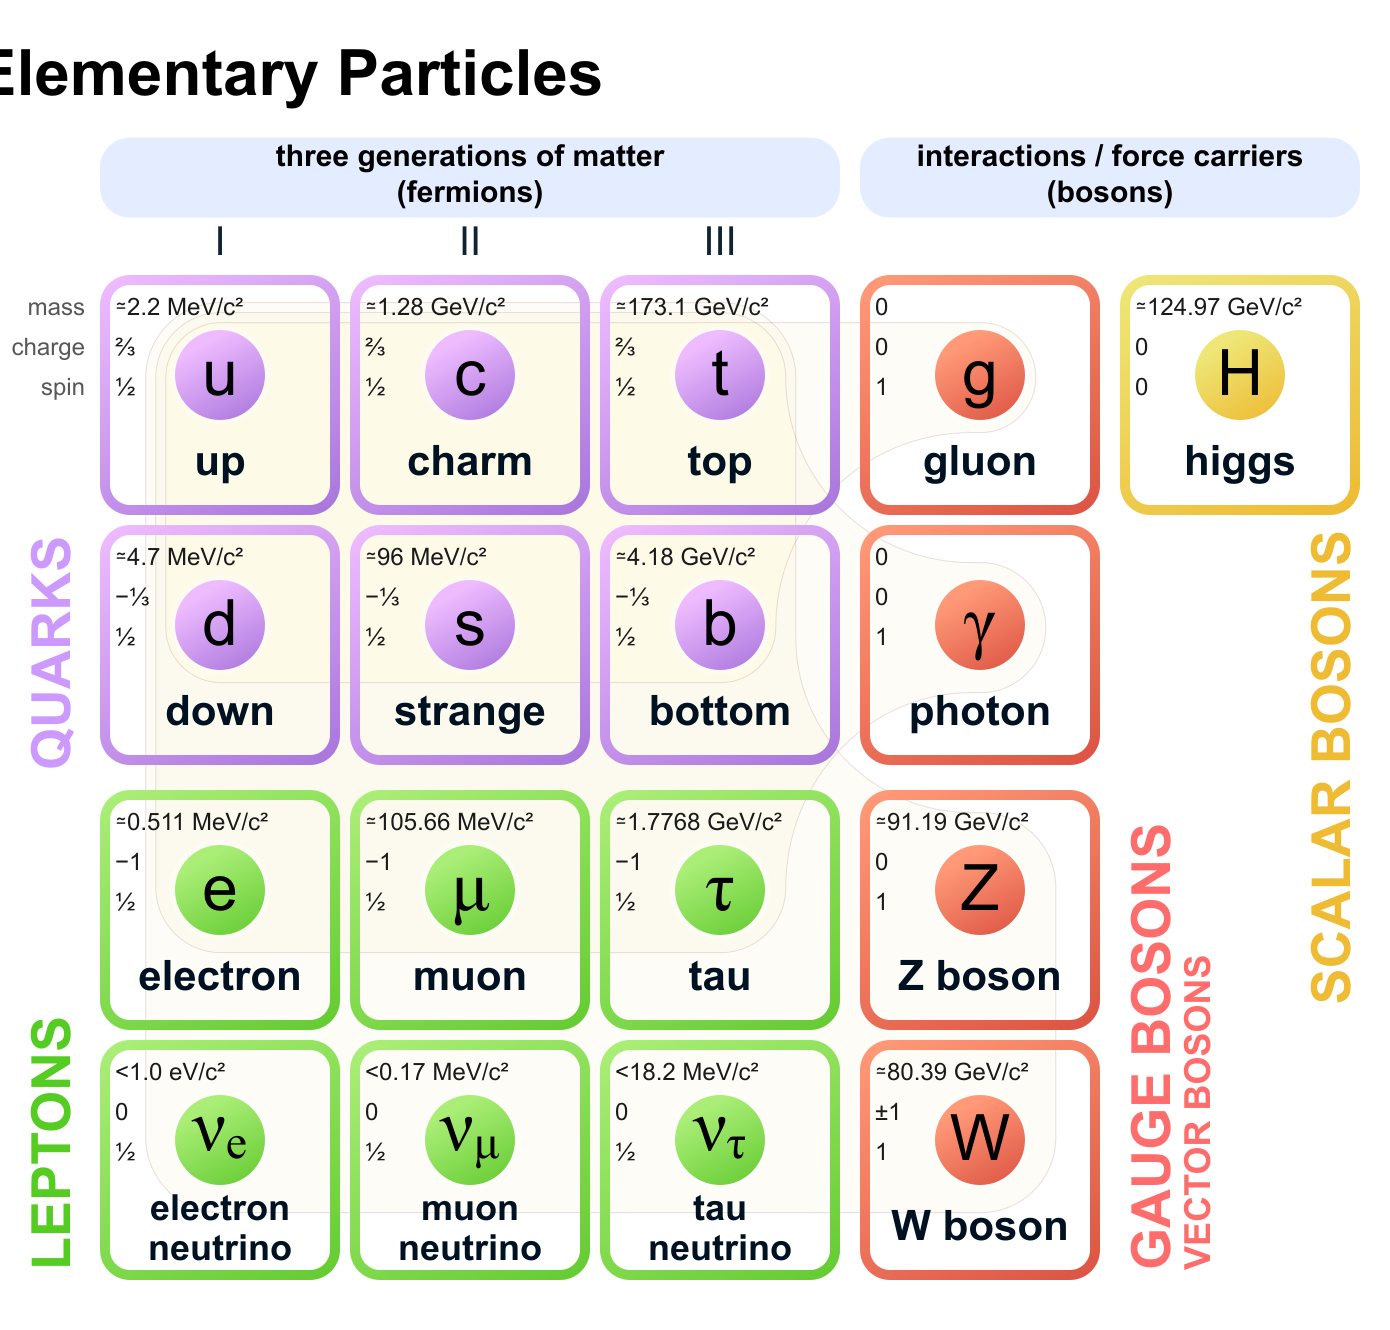
\includegraphics[width=0.7\textwidth]{figures/Fig14}
	\caption{The particle content of the Standard Model. Taken from \cite{SMImage}.}
	\label{Fig14}
\end{figure}
\section{Z boson production at the LHC}\label{chap2sec0}
Since the discovery of the Z and W bosons at the UA1 and UA2 experiments \cite{Arnison:1983rp,Arnison:1983mk,Banner:1983jy,Bagnaia:1983zx}, the Z boson has been the subject of multiple measurements in proton-proton and electron-positron colliders. The Z boson mass $m_Z=91.1875\pm0.0021$ GeV and its decay width $\Gamma_Z=2.4952\pm0.0023$ GeV have been measured to outstanding precision \cite{ALEPH:2005ab}. The braching ratios of the Z boson are well known; they are presented in Table \ref{Table0}.
\begin{table}[]
	\centering
	\begin{tabular}{cc}
		\hline
		\multicolumn{1}{|c|}{Decay mode} & \multicolumn{1}{c|}{Branching fraction (\%)} \\ \hline
		$e^+e^-$                         & $3.363\pm0.004$                              \\
		$\mu^+\mu^-$                     & $3.366\pm0.007$                              \\
		$\tau^+\tau^-$                   & $3.370\pm0.008$                              \\
		Invisible                        & $20.00\pm0.06$                               \\
		Hadrons                          & $69.91\pm0.06$                               \\ \hline
	\end{tabular}
	\caption{Z boson branching fractions. Number taken from \cite{PhysRevD.98.030001}.}
	\label{Table0}
\end{table}
In contrast to electron-positron colliders, the momentum of partons in proton-proton collisions is not precisely known. Thus, parton density functions (PDFs) are used to describe the proton structure in a phenomenological way. These functions are written as $f_{a/A}(x,Q^2)$ and represent the probability density for a parton $a$ to have a fraction $x=\frac{p_a}{p_A}$ of the proton momentum $p_A$. $Q$ is the energy scale of the scattering process. In this case, the cross section of two protons going to a final state $n$ will be
\begin{equation}
	\sigma_{p_Ap_B\to n}=\sum_{q}\int dx_adx_b f_{a/A}(x_a,Q^2) f_{b/B}(x_b,Q^2)\times [\sigma_0+\alpha_s\sigma_1+\dots]_{ab\to n}.
\end{equation}
The sum is made over all the partons. $\sigma_0$ is the tree level parton-parton cross section and $\sigma_1$ are the QCD corrections to first order. A diagram of the production of the Z boson in proton-proton collisions is shown in Fig.\ref{Fig15}. 
\begin{figure}[h]
	\centering
	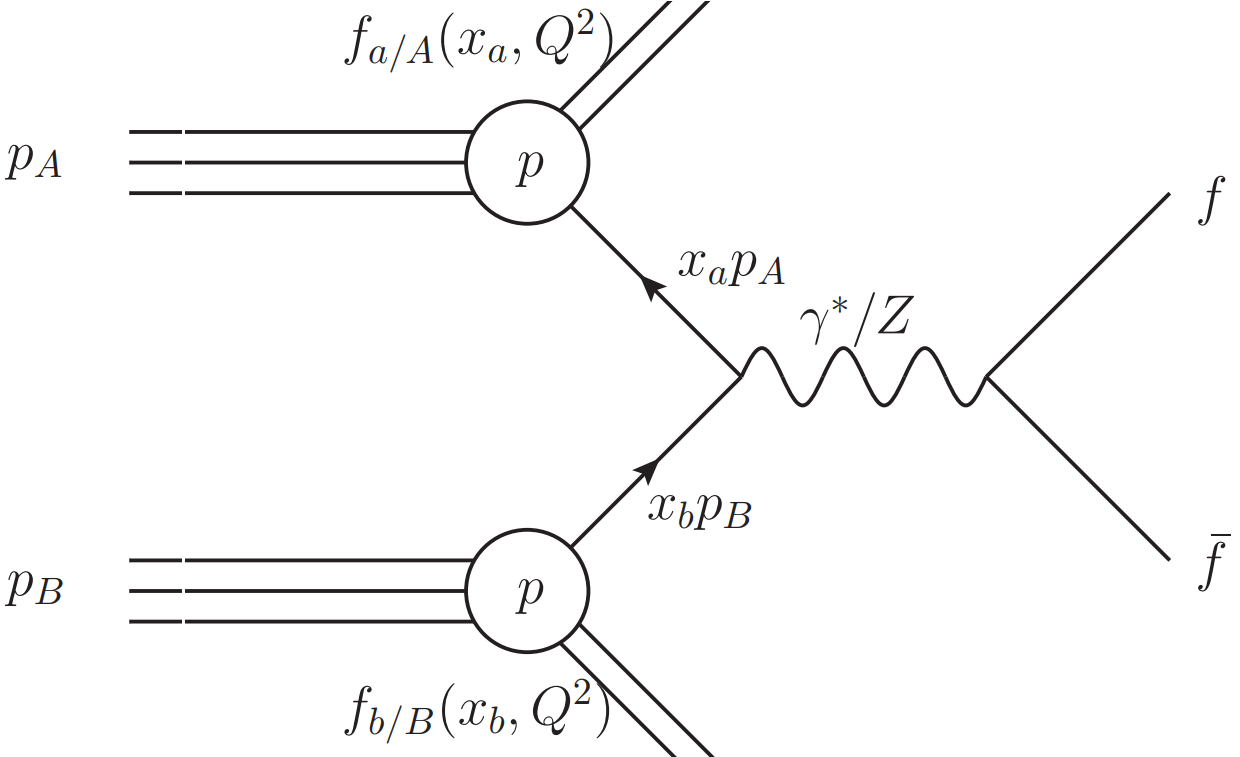
\includegraphics[width=0.6\textwidth]{figures/Fig15}
	\caption{Illustration of the production of a Z boson in pp collisions via quark-antiquark annihilation.}
	\label{Fig15}
\end{figure}
The main process contributing to Z boson production is the Drell-Yan process, where a quark-antiquark ($q\bar{q}$) pair annihilate, produce a Z boson and it subsequently decays into a pair of fermions. In this case, the transverse momentum ($\pt$) of the Z boson comes from the intrinsic $\pt$ of the partons. Nevertheless, this has been experimentally determined with a value of $<k_T>=0.76$ GeV \cite{Ellis:1991qj} and is not large enough to explain the measured Z boson $\pt$ distribution that peaks at a few GeV and has a tail that extends at values $\pt\gg m_Z$ \cite{Abbott:1999yd,Affolder:1999jh}.

To explain this kinematic feature we have to look at the other ways the Z boson can be produced in $pp$ collisions. First quark-gluon ($qg$) scattering, where the Z boson recoils against the quark radiated by the gluon in the initial state, this process is illustrated in Fig.\ref{Fig16a}. In the other hand, we could also have a gluon being radiated before $q\bar{q}$ annihilation takes place, having the Z boson recoiling against what is called \textit{initial state radiation} (ISR), as is shown in Fig.\ref{Fig16b}. High transverse momentum partons lead to the production of collimated showers of hadrons, called jets, that are subsequently detected as energy deposits in the calorimeters of the particle detectors. 
\begin{figure}[ht]
	\centering
	\subfloat[]{\label{Fig16a}{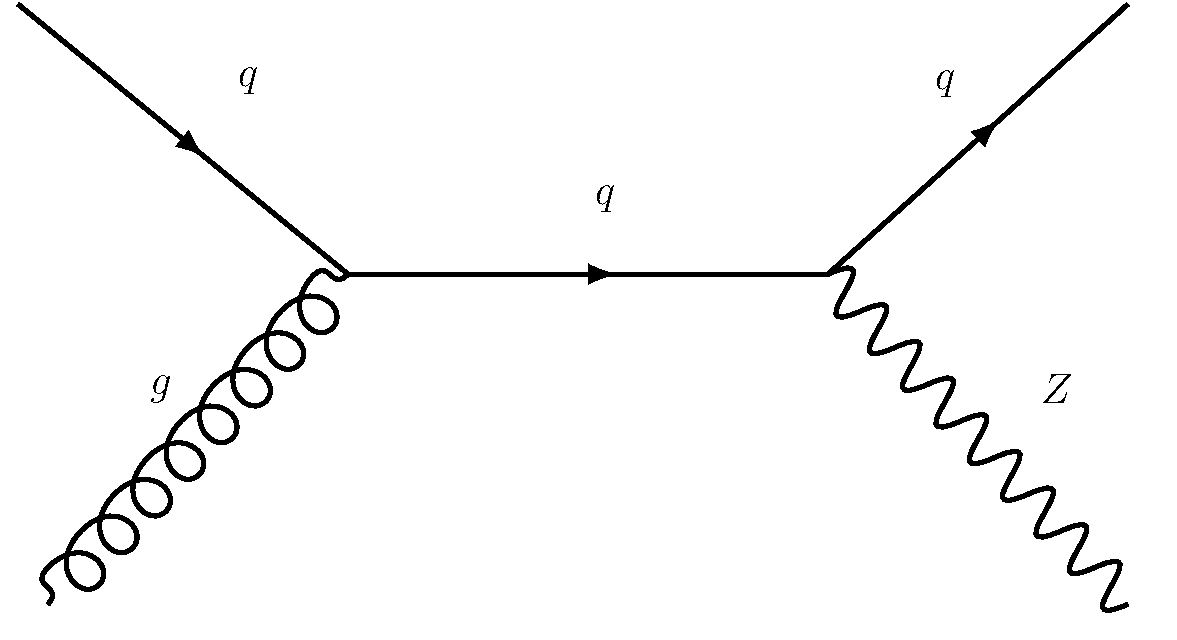
\includegraphics[width=0.50\textwidth]{figures/Fig16a}}}\hfill
	\subfloat[]{\label{Fig16b}{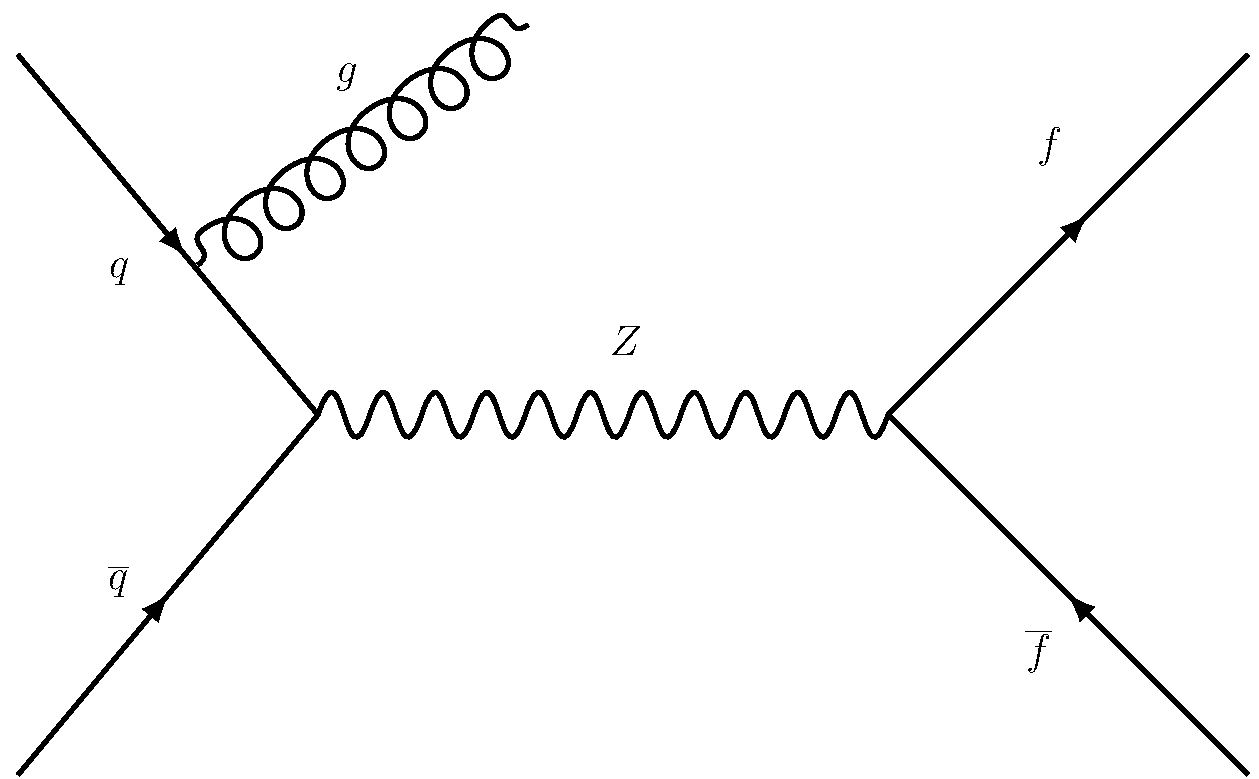
\includegraphics[width=0.50\textwidth]{figures/Fig16b}}}
	\caption{$qg$ Z boson production with FSR (a) and $q\bar{q}$ annihilation with gluon ISR (b).}
	\label{Fig16}
\end{figure}
\section{The Tau Lepton}\label{chap2sec1}
The tau is a spin-$\frac{1}{2}$ charged particle that belongs to the family of leptons. The first hints of the tau existence came from experiments conducted at the Stanford Linear Accelerator Center and Lawrence Berkeley National Laboratory \cite{PhysRevLett.35.1489}. They discovered 64 events of the form:
\begin{equation}
	e^+ + e^- \to e^\pm + \mu^\mp + \geq \text{2 undetected particles},
\end{equation}
for which there was no conventional explanation at the time. Later on, it was discovered that these events came from the production of a pair of new particles, two taus that subsequently decayed into one electron, a muon and four neutrinos. Events like,
\begin{equation}
e^+ + e^- \to \tau^+ \tau^- \to e^\pm + \mu^\mp + 4\nu,
\end{equation}	
were later explored to derive tau mass and spin, confirming the existence of a third generation of leptons. 
The tau has a mass of $1776.86 \pm 0.12$ MeV \cite{PhysRevD.98.030001}, which allows it to decay not only into the other lighter lepton generations (\textit{leptonic tau decays}), as shown on Fig.\ref{Fig1}  , but into hadrons. As we said on section \ref{chap2sec0} hadrons are particles made of quarks. All the decay channels of the tau containing hadrons in the final state are called \textit{hadronic tau decays}. Strictly speaking this is a semi-hadronic decay mode because of the presence of the neutrino. Nonetheless, from now on we will refer to these processes with the commonly used term \textit{hadronic tau decays}. An example of this decay mode is shown in Fig.\ref{Fig2}.
\begin{figure}[h]
	\centering
	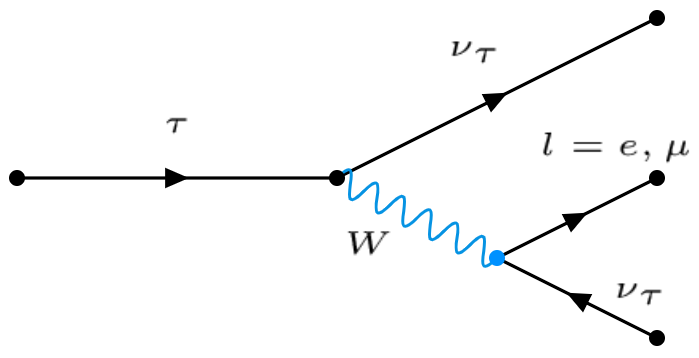
\includegraphics[width=0.6\textwidth]{figures/Fig1}
	\caption{Tau leptonic decay mode. Tau lepton is kinematically allowed to decay into muons or electrons, note that in this decay mode two neutrinos of different flavour are produced.}
	\label{Fig1}
\end{figure}
\begin{figure}[h]
	\centering
	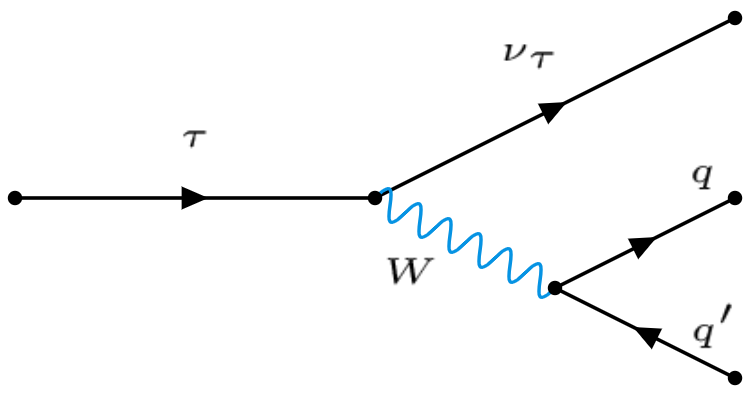
\includegraphics[width=0.6\textwidth]{figures/Fig2}
	\caption{Tau hadronic decay mode. The tau lepton is kinematically allowed only to decay into hadrons containing up, down and strange quarks. This results on final states containing multiple pions or kaons \cite{Davier_2006}.}
	\label{Fig2}
\end{figure}
The branching fraction for hadronic and leptonic tau decay modes is defined as
\begin{equation}
	\beta(\tau\to X\nu_\tau)=\frac{\Gamma(\tau\to X\nu_\tau)}{\Gamma_{\text{tot}}},
\end{equation}
where $X$ could be any number of leptons or hadrons and $\Gamma_{\text{tot}}$ is the total decay width for the tau. Naively, if we were to estimate it we could argue that the contribution from the hadronic decays triples the contribution for one of the leptonic modes. This is because in any hadronic decay, we would have to count 3 different diagrams, like the one in Fig.\ref{Fig2} because of the three colour possibilities for the quarks.

Thus, 
\begin{align}
\beta(\tau\to l\nu_l\nu_\tau)\approx 20\%& \hspace{1cm}l=e,\mu;
\\
\beta(\tau\to X\nu_\tau)\approx 60\%& \hspace{1cm} X=\text{hadrons+neutrinos}.
\end{align}
In fact, this naive estimation is not bad. Actual values for the leptonic branching ratios are \cite{PhysRevD.98.030001}:
\begin{align}
\beta(\tau\to e\nu_e\nu_\tau)&=17.82\pm 0.04\%
\label{eq6}
\\
\beta(\tau\to \mu\nu_\mu\nu_\tau)&=17.39\pm 0.04\%.
\end{align}
The reason for the difference in the estimation are the QCD corrections in the hadronic decays \cite{Pich:2013lsa}. The small difference between the leptonic branching fractions is due to the mass difference between the muon and the electron.

On the other hand, the hadronic decays of the tau are more varied and can contain many more particles in the final states. The vast majority of hadronic tau decays have charged or neutral pions in the final states, but more exotic decays including kaons also happen. Branching fractions for the most important tau hadronic decays are showed in Table \ref{Table1}.
\begin{table}[]
	\centering
\begin{tabular}{|c|c|}
	\hline
	Decay mode                     & Branching fraction \\ \hline
	$\pi^\pm \nu_\tau$             & 11.1 \%            \\ \hline
	$\pi^\pm \pi^0 \nu_\tau$       & 25.4\%             \\ \hline
	$\pi^\pm \geq 2\pi^0 \nu_\tau$ & 9.1\%               \\ \hline
	$3\pi^\pm \nu_\tau$            & 9.1\%               \\ \hline
	$3\pi^\pm \geq 1\pi^0 \nu_\tau$& 4.6\%               \\ \hline
	others						   & 5.5\%               \\ \hline
\end{tabular}
	\caption{Branching fractions for hadronic tau decay modes \cite{PhysRevD.98.030001}.}
	\label{Table1}
\end{table}
\section{Lepton Universality}\label{chap2sec2}
The SM predicts that all charged leptons $(e,\mu,\tau)$ interact via the electroweak force and explains that these interactions can be seen as the interchange of \textit{vector bosons}, the photon $(\gamma)$ and the W and Z bosons. Specifically, in the SM the form of the interaction does not depend on the lepton generation. This feature of the SM is called \textit{lepton universality} and is the fact that the couplings of the electrons, muons and taus to the electroweak bosons are identical. 

For instance, tau leptonic decay widths present a great opportunity to test lepton universality hypothesis. If we start considering muon decay, at low energies we can consider this process to be a point like interaction well described by Fermi theory \cite{FermiTheory}. In this case, if we approximate the electron and neutrinos as being massless particles, a dimensionally correct expression for the width is of the form
\begin{equation}
	\Gamma(\mu\to e+\nu_e +\nu_\mu)=KG_{F}^{2}m_{\mu}^{5},
\end{equation} 
where $G_F=1.1666\times 10^{-5} \text{ GeV}^{-2}$ is the Fermi coupling constant and $K$ is a constant that depends on the form of the interaction. If we assume that lepton universality holds, the respective widths for the tau leptonic decay modes, will have the form
\begin{align}
\Gamma(\tau\to e+\nu_e +\nu_\tau)&=KG_{F}^{2}m_{\tau}^{5},
\\
\Gamma(\tau\to \mu+\nu_\mu +\nu_\tau)&=\Gamma(\tau\to e+\nu_e +\nu_\tau),
\end{align}  
which explains why to a good approximation leptonic branching fractions for tau decay are equal. Moreover, we can obtain a relation between tau and muon lifetimes. We know that,
\begin{equation}
	\tau_l=\frac{1}{\Gamma_\text{Tot}}=\frac{\beta(l\to e\nu_e \nu_l)}{\Gamma(l\to e\nu_e \nu_l)},
	\label{eq11}
\end{equation}
also that $\beta(\mu\to e\nu_e \nu_\mu)=1$ and taking into account eq.(\ref{eq6}) we can take the ratio between eq.(\ref{eq11}) for $l=\tau ,\mu$ to obtain
\begin{equation}
\frac{\tau_\tau}{\tau_\mu}=\frac{\beta(\tau\to e\nu_e \nu_\tau)}{\beta(\mu\to e\nu_e \nu_\mu)}\left(\frac{m_\mu}{m_\tau}\right)^5=(1.328\pm 0.004)\times 10^{-7}.
\end{equation}
This is consistent with the experimental lifetimes ratio of $(1.3227\pm 0.0005)\times10^{-7}$ \cite{Martin:1992rg}. This agreement on lifetimes that differ by seven orders of magnitude is a good proof that lepton universality holds on W decays at the tau mass scale.

Very precise tests of LU have been done by $e^-e^+$ colliders (LEP1, SLC and LEP2). Measurements of the ratios between the leptonic decay widths of the Z boson have been performed and are consistent with the SM \cite{ALEPH:2005ab}:
\begin{align}
	\frac{\Gamma(Z\to\mu^+\mu^-)}{\Gamma(Z\to e^+e^-)}=1.0009\pm 0.0028,
	\\
	\frac{\Gamma(Z\to\tau^+\tau^-)}{\Gamma(Z\to e^+e^-)}=1.0019\pm 0.0032.
\end{align}
LU has also been tested in W boson decays. A combination of measurements made by different experiments of the branching fractions between the first two families of leptons are consistent with SM predictions \cite{Pich:2013lsa}:
\begin{equation}
\frac{\beta(W^-\to e^-\bar{\nu_e})}{\beta(W-\to \mu^-\bar{\nu_\mu})}=1.004\pm 0.008.
\end{equation}
However, measurements including the third lepton family, apart from being less precise due to the more challenging reconstruction of the $\tau$ lepton final states are in tension with SM \cite{Schael:2013ita}:
\begin{align}
\frac{\Gamma(W^-\to\tau^-\bar{\nu_\tau})}{\Gamma(W^-\to e^-\bar{\nu_e})}=1.063\pm 0.027,
\\
\frac{\Gamma(W^-\to\tau^-\bar{\nu_\tau})}{\Gamma(W^-\to \mu^-\bar{\nu_\mu})}=1.070\pm 0.026.
\end{align}
These results show that LU between the two first lepton family holds with a precision of 0.3\% and 0.8\% in Z and W decays respectively. Constraints between the third and the other two generations of leptons are of similar precision on Z boson decays (0.3\%), but ten times worse for W boson decays (3\%) and somewhat in tension with SM prediction. %%An example of this is a measurement exhibiting a tension of 2.6 $\sigma$ from the SM expectation \cite{Schael:2013ita}:
%%\begin{equation}
	%%\frac{2\Gamma(W^-\to\tau^-\bar{\nu_\tau})}{\Gamma(W^-\to e^-\bar{\nu_e})+\Gamma(W^-\to %%\mu^-\bar{\nu_\mu})}=1.066\pm 0.025.
%%\end{equation}  


Furthermore, measurements from LHCb, BaBar and Belle experiments have shown consistent deviations from the SM predictions \cite{Ciezarek_2017}. These experiments have independently measured a deviation on $\bar{B}$ meson semi-leptonic branching ratios, specifically:
\begin{align}
	R_D&=\frac{\beta(\bar{B}\to D\tau^-\bar{\nu}_\tau)}{\beta(\bar{B}\to De^-\bar{\nu}_e)}
	\\
	R_{D^\star}&=\frac{\beta(\bar{B}\to D^\star\tau^-\bar{\nu}_\tau)}{\beta(\bar{B}\to D^\star e^-\bar{\nu}_e)}.
\end{align}
The combined results for the different experiments are shown in Fig.\ref{Fig3}. These measurements represent a 3.08 $\sigma$
 deviation from the SM predictions, but even though they represent a hint of new physics, higher statistical precision will be needed to confirm this results. Future analysis from experiments like LHCb and Belle II with larger available datasets will be very important to untangle this situation.
 \begin{figure}[h]
 	\centering
 	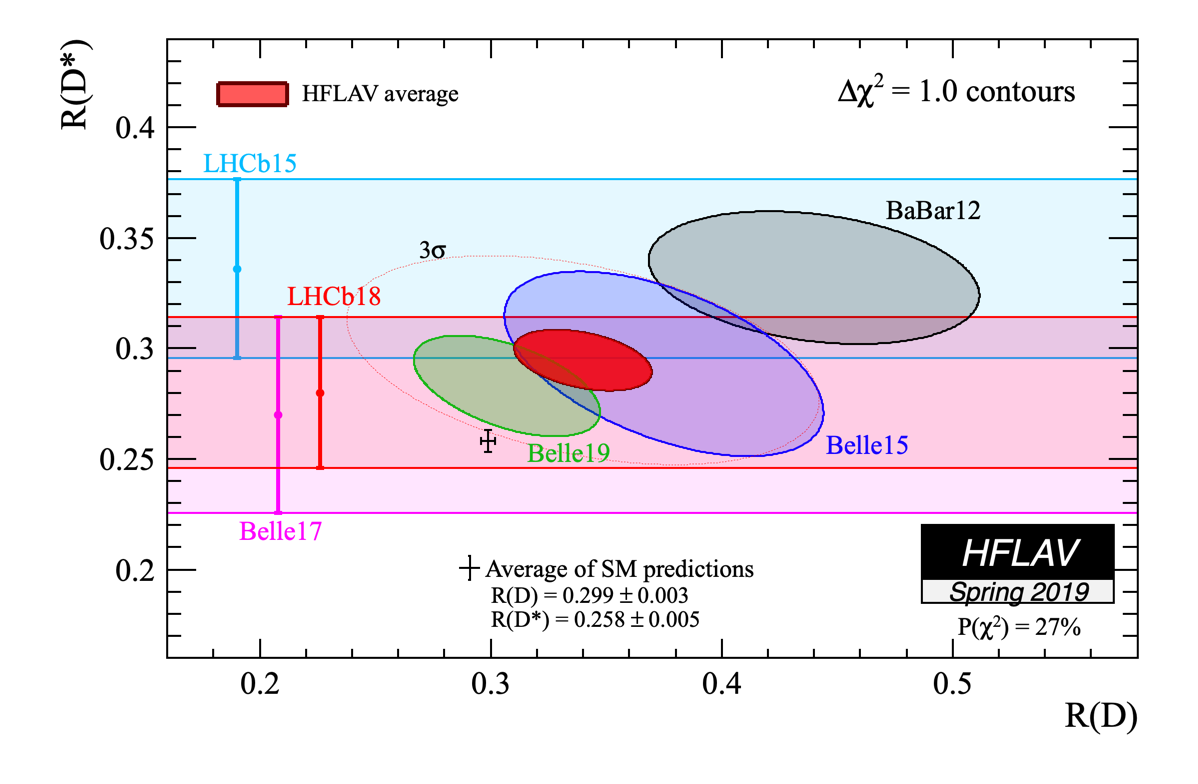
\includegraphics[width=0.7\textwidth]{figures/Fig3}
 	\caption{Combined results from BABAR, Belle and LHCb with 1-$\sigma$ contour. The average calculated by the Heavy Flavour Averaging Group \cite{HFAG}  is compared with the SM predictions.}
 	\label{Fig3}
 \end{figure}
    \chapter{Analysis}\label{chap1}
At the begining of this chapter, a review of the ATLAS detector at the LHC and a description of the reconstruction and identification of hadronic Tau decays on ATLAS are discussed. The last sections are devoted to describe the Analysis methodology of using $Z\to\tau\tau$ events to measure Monte Carlo correction factors for Tau identification algorithms on the high-$p_T$ region.

\section{The LHC and the ATLAS experiment}

\section{Tau Reconstruction and Identification on the ATLAS detector}
Leptonically decaying taus ($\tau_\text{lep}$), may have a higher impact parameter and tend to have a softer $p_T$ spectrum compared with prompt W or Z boson decays to muons or electrons. This variables are not sufficient in principle to differentiate between $\taul$ and prompt muons or electrons. In the case of hadronically decaying taus ($\tau_\text{had}$), as we will see, there are a lot more variables we could use to tag the presence of a $\tauh$.

As we saw in section \ref{chap2sec1}, $\tauh$ decays can be classified in 1-prong or 3-prong, depending on the number of charged particles in the decay. A detailed review of the reconstruction procedure is discussed on REF TAU RECO. $\tauh$ candidates are seeded by jets using the anti-$k_t$ algorithm REF ANTI KT, with a distance parameter of 0.4. Jets are required to have $p_T>10$ GeV and $|\eta|<2.5$. Candidates between the barrel and forward calorimeter ($1.37<|\eta|<1.52$) are excluded due to poor instrumentation in this region.

The axis of the seed jet is defined by the energy-weighted barycentre of all clusters of calorimeter cells, called \textit{TopoClusters} REF TOPO CLUSTERS. The $\tauh$ vertex is defined as the vertex with the highest $p_T$-weighted fraction of all tracks with $p_T>0.5$ GeV within a cone of $R=0.2$ around the seed jet axis. Tracks within a cone of $R=0.4$ are classified with a set of boosted decision trees (BDTs) into core and isolation tracks, the number of core tracks defines the number of prongs. Candidates with neither one or three tracks are rejected. Additionally, the sum of the charge of the tracks is required to be $\pm 1$.     

\section{Monte Carlo Samples}

\section{The Collinear Approximation}

\section{Event Selection}
    \chapter{Results}\label{chap:approach}
The approach usually starts with the problem definition and continues with what you have done. Try to give an intuition first and describe everything with words and then be more formal like `Let $g$ be ...'.
\section{$\mu\tau$ Final state}
\section{$e\tau$ Final state}
Start with a very short motivation why this is important. Then, as stated above, describe the problem with words before getting formal.

\section{Monte Carlo and data discrepancies}


    \chapter{Conclusions and prospects}\label{chap:experiments}

\input{figures/experiments/figExample}
\begin{table}[ht]
\centering
% spacing in table
\ra{1.3}
\begin{tabular}{@{}lr@{}}
  \toprule
  Type & Accuracy\\ \midrule
  A    & 82.47 $\pm$ 3.21 \\
  B    & 78.47 $\pm$ 2.43 \\
  C    & 84.30 $\pm$ 2.35 \\
  D    & 86.81 $\pm$ 3.01 \\
  \bottomrule
\end{tabular}

    \caption[Table caption]{\textbf{Table caption.} foo bar...\\}
    \label{tab:accuracy}
\end{table}
    %\input{chapters/6-conclusions}
    %\input{chapters/7-acknowledgments}
    
    % If you want a list of your ToDos at the end of the document
    % don't forget to remove before submission!
    %% place it somewhere in the document
\chapter*{ToDo Counters}
\newcounter{ct}%
To Dos: \arabic{todos}; \hspace{1em}%
\setcounter{ct}{0}%
\whiledo {\value{ct} < \value{todos}}%
{%
	\stepcounter {ct}%
    \ref{todo \thect}%
	\ifnum\value{ct} = \value{todos}{}\else{, }\fi
}

Parts to extend: \arabic{extends}; \hspace{1em}%
\setcounter{ct}{0}%
\whiledo {\value{ct} < \value{extends}}%
{%
	\stepcounter {ct}%
	\ref{extend \thect}%
	\ifnum\value{ct} = \value{extends}{}\else{, }\fi
}

Draft parts: \arabic{drafts}; \hspace{1em}%
\setcounter{ct}{0}%
\whiledo {\value{ct} < \value{drafts}}%
{%
	\stepcounter {ct}%
	\ref{draft \thect}%
	\ifnum\value{ct} = \value{drafts}{}\else{, }\fi
}


    \bibliographystyle{ieeetr}
    \bibliography{bib/topic1,bib/topic2}
    % bibliography is not in the table of contents per default, add it manually
    % enable the \renewcommand for german header
    % \renewcommand{\bibname}{Literaturverzeichnis}
    \addcontentsline{toc}{chapter}{Bibliography}
    \newpage
    \thispagestyle{empty}
    \mbox{}


\end{document}
